\documentclass[a4paper,10pt]{article}

\setlength{\parindent}{0mm}
\setlength{\oddsidemargin}{-5mm}
\setlength{\evensidemargin}{-5mm}
\setlength{\textwidth}{165mm}
\setlength{\textheight}{230mm}
\setlength{\topmargin}{-10mm}
\setlength{\marginparwidth}{15mm}
\setlength{\marginparsep}{7mm}
\usepackage{float}

%Include some packages which give certain fonts, graphics capabilities, etc
\usepackage{graphicx}% Include figure files
\usepackage{dcolumn}% Align table columns on decimal point
\usepackage{color}% bold math
\usepackage{bm}% bold math
\usepackage[caption=false]{subfig}
\usepackage{listings}

%% Define the names of come colours you can use in your report.
\usepackage[usenames]{color}
%provide smart hyperlinks in your document
\newcommand{\cross}{\ding{55}}



\begin{document}



% remove the following for publication
\begin{figure}
\leftline{\hfill PHYS281 Final Report}
\end{figure}




% Front matter 
\title{A simulation of an N bodied System in Python  }
\author{Samuel Hedges}
\date{01/12/21}
 \maketitle
\begin{abstract}
The effectiveness of a Simulation, in the python soft wear, of the Inner solar system using the Euler and Euler-Cromer Numerical Approximations was carried out and found that the simulation wasn't that effective at simulating the solar system when compared to NASA simulations, although it is able to generate a working solar system with the proper elliptical orbits.
\end{abstract}
\newpage

\section{Introduction and Theory}
This project was to simulate gravitational systems using the python coding language \cite{Python}. Through implementation of the Euler \cite{Euler} and Euler-Cromer \cite{Euler-Cromer} numerical approximations, and use of Newton's Law of Universal Gravitation\cite{Universal Grav}, Newton's Laws of motion\cite{university physics} and the Conservation Laws for Energy and Momentum; the simulation can now accurately model the inner solar system. For all this project NumPy was used for its array function, ability to preform vector operations and to make save states of the attributes of the particles passed through the particle class. \cite{NumPy}

\subsection{Physical Laws Used}
Newton's Law of Universal Gravitation states that all particles enact on all other particles in the Universe with an attractive force that is proportional to the product of the masses of the particles and inversely proportional to the square of the distance between them. The constant of proportionality is known as the Universal Gravitational Constant, and it has been worked out subsequently through experimental data.This can be written out in the form of an equation:

\begin{equation}
  F = \frac{Gm_{1}m_{2}}{r^{2}} \label{eq:Gravitational Force}
\end{equation}

Where $\boldsymbol F$ is the Force on the particles in Newtons, $\boldsymbol G$ is the universal gravitational constant (whose value has been subsequently worked out experimentally), $\boldsymbol {m_{1} /  m_{2}}$ are the masses of the two particles, and $\boldsymbol r$ is the magnitude of the distance between the two particles. This allows the simulation to model effectively the interplanetary interactions via coding the above into python

Newton's First law of motion tells us that the rate of change of velocity multiplied by mass is proportional to the force on the body. This equation can be rearranged to get the following equation:

\begin{equation}
  \frac{d^{2}x}{dt^{2}} = \frac{F}{m} \label{eq:Newton's First Law of Motion}
\end{equation}

This explains that the Force on the bodies can be changes into an acceleration by diving it by the mass. This was used to find the acceleration of the body that could be fed into one of the numerical methods to update the position and velocity of the body. This acceleration could be found by dividing the sum of the gravitational forces on a body by the mass of that body. In principle this meant that the acceleration of the body was found via:

\begin{equation}
F = \frac{Gm_{1}}{r^{2}} \label{eq:Gravitational Acceleration}
\end{equation}

Where $\boldsymbol F$ is the Force on the particles in Newtons, $\boldsymbol G$ is the universal gravitational constant, $\boldsymbol r$ is the magnitude of the distance between the two bodies, and $\boldsymbol m_1$ is the mass of the body which causes the acceleration i.e. For the orbit of the moon $\boldsymbol m_1$ would be the mass of the earth \cite{The earth moon system}.

In analysing the accuracy of the simulation a number of Conservation Laws were used. The Law of conservation of energy states that "Energy in an isolated system is conserved over time". The model Inner solar system can be considered to be an isolated system therefore if there is an assumption that the two stores of energy are kinetic and gravitational potential energy; the sum of these two sources (summed over all bodies) should be conserved over time. the total energy in the system can therefore be tested to test the accuracy of the Model produced. Momentum is also a conserved quantity in a closed system. This conservation can be implied by Newton's second law of motion \cite{SLOM} that states "The rate of change of a body's momentum is equal to the net force on the body".
This can be written as the following equation:
\begin{equation}
    F = \frac {d}{dt}\boldsymbol{mv} \label{eq:Newton's Second Law of Motion}
\end{equation}
Where $\boldsymbol F$ is the force on the body; $\boldsymbol m$ the mass of the body and $\boldsymbol v$ the velocity of the body.
This mean the model can be tested against how well it conserves Momentum as well as energy.

\subsection{Numerical Approximations} 

The Euler Method is a way of solving an ordinary differential equation using first order numerical values and the initial value of the ordinary differential equation. In this simulation it is being used to update the position and velocity when an acceleration is known.


\begin{equation}
    x_{n+1} \approx x_{n} + v_{n}\Delta t \label{eq:Euler 1}
\end{equation}
\begin{equation}
    v_{n+1} \approx v_{n} + a_{n}\Delta t\label{eq:Euler 2}
\end{equation}
where $x$ is a position of a body, $v$ is a velocity of a body, $a$ is an acceleration of a body, and $\Delta t$ is a small-time interval.

The Euler Method is being applied such that there is an assumption that in the small-time period $\Delta t$ there is a near constant acceleration. This method was concluded on via taking the first few terms of the Taylor series expansion \cite{taylor series} and thus each time it is iterated over we expect an error in the order of ${\Delta t}^2$.

The Euler-Cromer method (also known as the semi-implicit) is a modification of the Euler Method altered to solve Hamiltonian Equations. In this method you iterate over the velocity before then iterating over the acceleration.
\begin{equation}
    v_{n+1} \approx v_{n} + a_{n}\Delta t\label{eq:Euler 2}
\end{equation}
\begin{equation}
    x_{n+1} \approx x_{n} + v_{n}\Delta t \label{eq:Euler 1}
\end{equation}
 The Euler Cromer-Method will be less accurate over all picking up an error of the order ${\Delta t}^2$, but due to being based on Hamiltonian Mechanics will be better at conserving Kinetic energy in the system.


\section{Results}
The simulation was run for 100,000 steps of 3,600 seconds. The 100,000 steps was used as it encompassed the whole orbit of all the celestial bodies programmed in the simulation. This meant that if there was a significant error with of the bodies movements it could be located and dealt with. 
The 3,600 time step was chosen as it is suitably large to not need a lot of iterations without being too large that the error of the system would be unmanageable (It is also the length of an hour in seconds meaning that it could be seen down to the hour how the system was evolving). Both the Euler and Euler-Cromer numerical methods were tested under these conditions. The data was saved to a .npy file type \cite{.npy} and accessed using the NumPy's load feature.



\subsection{Conservation of Energy and Momentum}
Twenty equally spaced measurements of the total momentum and total energy in the system were taken. These were then plotted using a soft wear called QTIPlot \cite{QTIPlot}.

The following is the Table of results contains the data from both the Euler and Euler-Cromer Numerical approximations used

\begin{table}[htbp]
\begin{center}
\begin{tabular}{|c|c|c|c|c|}
\hline 
Time & \multicolumn{2}{|c}{Total Momentum in the sysetm} & \multicolumn{2}{|c|}{Total Energy in the system} \\
\hline
Both Methods  & Euler Method & Euler-Cromer Method & Euler Method & Euler-Cromer Method \\
Seconds [$10^{6}]$ & Joules [$10^{28}$]& Joules [$10^{28}$]& $kgms^{-1}$ [$10^{42}$]& $kgms^{-1}$ [$10^{42}$]\\
\hline
   0 & 1.5032633875676 & 1.5032633875676 & -5.384436251007617 &  -5.384436251007617\\ 
   18 & 1.503312404267 & 1.503312404267 & -5.384485679968 &  -5.384485679968\\
   36 & 1.503361430136 & 1.503361430149 & -5.384535107323 &  -5.384535107384\\
   54 & 1.503410465168 & 1.503410465207 & -5.384584533014 &  -5.384584533198\\
   72 & 1.503459509359 & 1.503410465207 & -5.384633956983 &  -5.384633957349\\
   90 &1.503508562703 & 1.503508562834 & -5.38468337917 &  -5.384683379781\\
   108 & 1.503557625196 & 1.503557625393 & -5.384732799517 &  -5.384732800434\\
   126 & 1.503606696834 & 1.503606697109 & -5.384782217965 &  -5.384782219249\\ 
   144 & 1.50365577761 & 1.503655777977 & -5.384831634454 &  -5.384831636168\\
   162 & 1.50370486752 & 1.503704867992 & -5.384881048927 &  -5.384881051131\\
   180 & 1.503753966558 & 1.503753967149 & -5.384930461324 &  -5.38493046408\\
   198 & 1.503803074721 & 1.503803075444 & -5.384979871587 &  -5.384979874956\\
   216 & 1.503852192003 & 1.503852192871 & -5.385029279655 &  -5.3850292837\\
   234 & 1.503901318399 & 1.503901319426 & -5.385078685471 &  -5.385078690252\\ 
   252 & 1.503950453903 & 1.503950455103 & -5.385128088975 &  -5.385128094555\\ 
   270 & 1.503999598512 & 1.503999599897 & -5.385177490107 &  -5.385177496549\\
   288 & 1.504048752219 & 1.504048753804 & -5.38522688881 &  -5.385226896174\\
   306 & 1.504097915021 & 1.504097916818 & -5.385276285023 &  -5.385276293372\\
   324 & 1.504147086912 & 1.504147088935 & -5.385325678687 &  -5.385325688084\\ 
   342 & 1.504196267886 & 1.50419627015 & -5.385375069744 &  -5.38537508025\\ 
   360 & 1.50424545794 & 1.504245460457 & -5.385424458134 &  -5.385424469811\\
\hline 
\end{tabular}
\end{center}
\caption{\label{table:Magnitude of Conserved Quantities} This is a table of the value of the conserved quantities and how they changes over time}
\end{table}


\begin{figure}[]
   \centering
   \subfloat[Euler Method Momentum change]{
   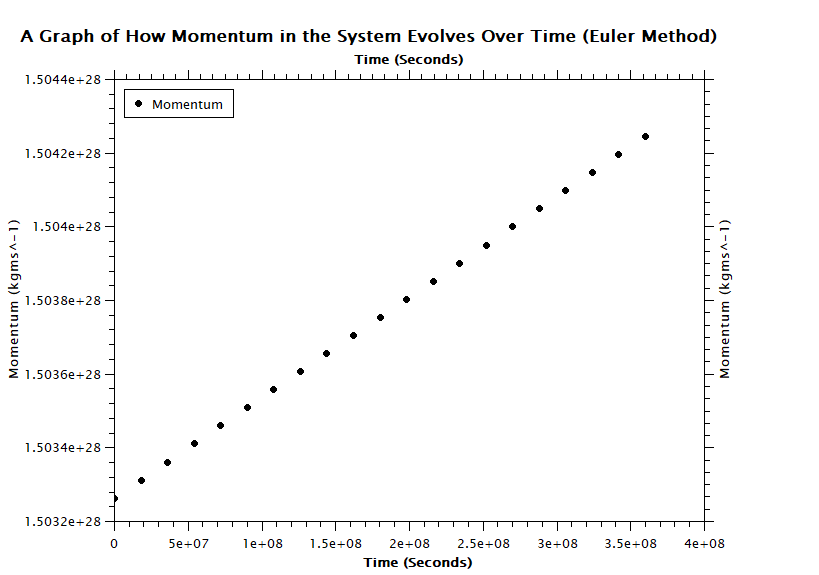
\includegraphics[width=0.5\columnwidth]{Euler Method/A Graph of How Momentum in the System Evolves Over Time (Euler Method).png}}
   \subfloat[Euler-Cromer Method Momentum change]{
   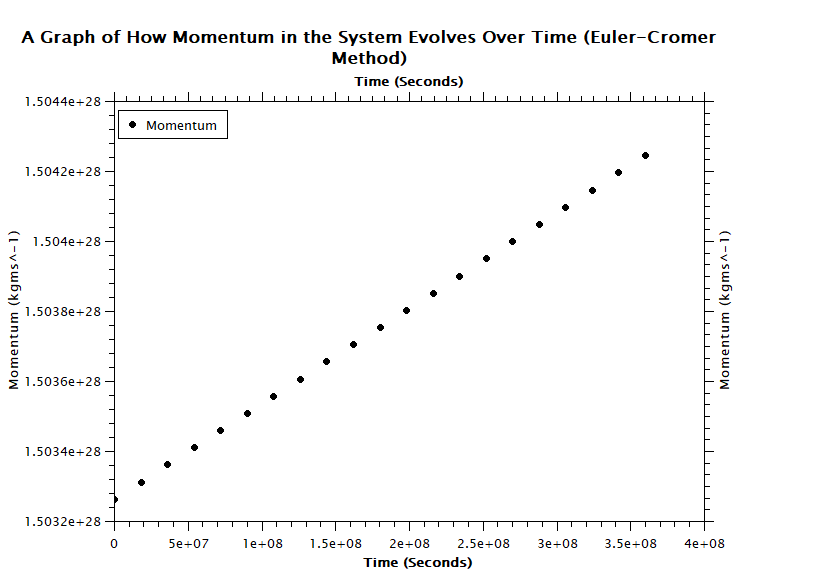
\includegraphics[width=0.5\columnwidth]{Euler-Cromer Method/A Graph of How Momentum in the System Evolves Over Time (Euler-Cromer Method).png}}
   \caption{Here are the Plots of how the two Methods and how the momentum in the system changes under both Methods}
   \label{plot:linear}
\end{figure}

\begin{figure}[]
   \centering
   \subfloat[Euler Method Energy chnage]{
   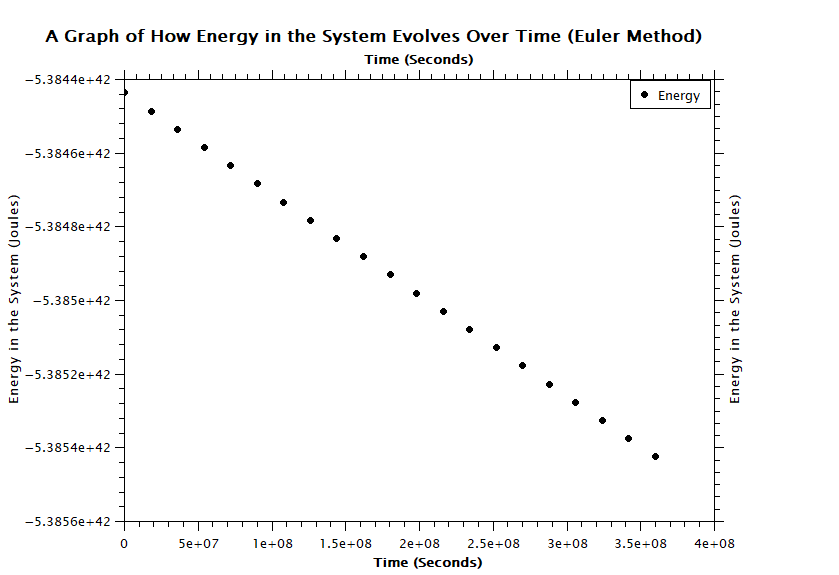
\includegraphics[width=0.5\columnwidth]{Euler Method/A Graph of How Energy in the System Evolves Over Time (Euler Method).png}}
   \subfloat[Euler-Cromer Method Energy change]{
   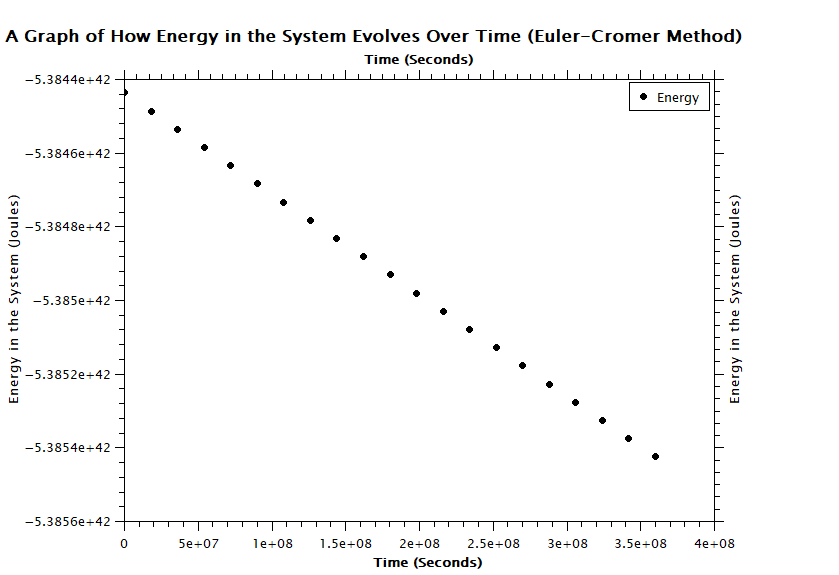
\includegraphics[width=0.5\columnwidth]{Euler-Cromer Method/A Graph of How Energy in the System Evolves Over Time (Euler-Cromer Method).png}}
   \caption{Here are the Plots of how the two Methods and how the energy in the system changes under both Methods}
   \label{plot:linear}
\end{figure}
\newpage
The Table and Graphs provide clear evidence that these conserved quantities, energy and momentum, are not perfectly conserved under the Euler and Euler-Cromer methods. The reasoning for this is the methods use a small-time step (that has been referred to as $\Delta t$ in the Numerical Methods) to calculate the position and velocity of the planets for both the Euler and Euler-Cromer Methods. This small-time step will approximate the infinitesimal time step that we would usually use. This has resulted in the expected error of a factor of $\Delta t^{2}$. as there will be some error from using an approximation to integrate the velocity and position with relation to the acceleration.

The percentage change in both momentum and velocity can be calculated using:
\begin{equation}
   \frac {\Delta \boldsymbol{p}}{\boldsymbol{p_{0}}} 
\end{equation}
and 
\begin{equation}
   \frac {\Delta {U}}{{U_{0}}}
\end{equation}
Where $\Delta \boldsymbol{p}$ is the absolute value of the change in Momentum; $\boldsymbol{p_{0}}$ is the momentum in the system at time $t=0$; $\Delta {U}$ is the absolute value of the change in Energy and ${U_{0}}$ is the Energy in the system at time $t=0$.

Through completion of the calculations it is found that for the Euler Method had a momentum percentage difference of $6.53292*10^{-4}\%$ and Energy percentage difference of $1.83530*10^{-4}\%$ .The Euler-Cromer Method had a momentum percentage difference of $6.53294*10^{-4}\%\%$ and Energy percentage difference of $1.83532*10^{-4}\%$. From these results it can be argued that the simulation does effectively model the inner solar system; the reason being that for both methods we see a percentage change orders of magnitude smaller than the original value and therefore can be seen to go to zero. This shows that the simulation built is an effective one as it is able to reasonably conserve values which we know to be conserved in our universe. 

Out of the two methods we see that the Euler-Cromer Method was worse for both energy and momentum conservation having a larger percentage difference for both. Despite this there is not enough evidence to state it is significantly worse than the Euler method as they both agreed to 8 significant figures for both energy and momentum. This can be considered very accurate, and it is unlikely that such accuracy would be required in a non-specialist environment.

\subsection{Comparison NASA's Results}
Using NASA's Jet Propulsion Laboratory (Which will be abbreviated to JPL from this point onwards) Horizon page \cite{} the simulation can be tested against an accurate ephemeris generated by NASA. Two bodies, Earth and Venus were chosen for this test so that the position and velocity could be tested against the results calculated by NASA.

\begin{table}[htp!]
\begin{center}
\begin{tabular}{|c|c|c|}
\hline 
Time & \multicolumn{2}{|c|}{Predicted Position of the Earth}  \\
\hline
  & NASA's JPL & Simulation\\
Weeks & metres & metres \\
\hline
   0 & (3.99213E+10, 1.42077E+11, 1.85607E+04) &  (3.99213E+10, 1.42077E+11, 1.85607E+04) \\ 
   1 & (2.20545E+10, 1.45944E+11, 1.86845E+07) & (4.0026E+10, 1.4211E+11, 1.85642E+07)   \\
   2 & (3.84305E+09, 1.47606E+11, 1.82317E+07 & (4.01308218E+10, 1.42135228E+11 1.85677530e+07)  \\
   3 & (-1.44473, 1.47041E+11, 1.83838E+07) & (4.02355365E+10 1.42164505E+11 1.85712820E+07)   \\
   
\hline 
\end{tabular}
\end{center}
\caption{\label{table:Magnitude of Conserved Quantities} This table shows a side by side comparison of NASA's JPL values of The Earth's position to the values given by the simulation for a 3-week period (starting 06/12/21 and ending 27/12/21). For this the Simulation used the Euler Method}
\end{table}

\begin{table}[htp!]
\begin{center}
\begin{tabular}{|c|c|c|}
\hline 
Time & \multicolumn{2}{|c|}{Predicted Velocity of the Earth} \\
\hline
  & NASA's JPL & Simulation \\
Weeks & metres per second & metres per second\\
\hline
   0 & (-2.9105E+04, 8.19579E+03, 9.77294E-01) & (-2.91059E+04, 8.19579E+03, 9.77294E-01) \\ 
   1 & (-2.99009E+04, 4.58046E+03, -5.56419E-01) & (2.90997222E+04, 8.17468452E+03, 9.78288356E-01)  \\
   2 & (-3.02493E+04, 9.10643E+02, -5.53589E-01) & (2.90935706E+04, 8.15359479E+03, 9.79281032E-01) \\
   3 & (-3.01609E+04, -2.78174E+03, 1.16555) & (2.90874E+04, 8.13253E+03, 9.80272E-01) \\
   4 & (-2.96112E+04, -6.46139E+03, 1.54112) & (2.90812E+04, 8.11148E+03, 9.81263E-01)\\
   
\hline 
\end{tabular}
\end{center}
\caption{\label{table:Magnitude of Conserved Quantities} This table shows a side by side comparison of NASA's JPL values of The Earth's velocity to the values given by the simulation for a 3-week period (starting 27/12/21 and ending 03/01/22). For this the Simulation used the Euler Method}
\end{table}
\begin{table}[htb!]
\begin{center}
\begin{tabular}{|c|c|c|}
\hline 
Time & \multicolumn{2}{|c|}{Predicted Position of the Venus}  \\
\hline
  & NASA's JPL & Simulation\\
Weeks & metres & metres \\
\hline
   0 & (6.29492E+10, 8.73986E+10, -2.48822E+09) & (6.29492E+10, 8.73986E+10, -2.48822E+09)  \\ 
   1 & (4.47244E+10, 9.81406E+10, -1.28907E+09) & (6.284733e+10,  8.74728e+10, -2.41927e+09)\\
   2 & (2.47294E+10, 1.05124E+11, -3.93386E+07) & (6.27453e+10,  8.75469e+10, -2.35032e+09)\\
   3 & (3.73007E+09, 1.08067E+11, 1.21287E+09) & (6.26433e+10,  8.76209e+10, -2.28136e+09)   \\
   
\hline 
\end{tabular}
\end{center}
\caption{\label{table:Magnitude of Conserved Quantities} This table shows a side by side comparison of NASA's JPL values of The Venus' position to the values given by the simulation for a 3-week period (starting 06/12/21 and ending 27/12/21). For this the Simulation used the Euler-Cromer Method}
\end{table}

\begin{table}[htb!]
\begin{center}
\begin{tabular}{|c|c|c|}
\hline 
Time & \multicolumn{2}{|c|}{Predicted Velocity of the Venus} \\
\hline
  & NASA's JPL & Simulation \\
Weeks & metres per second & metres per second\\
\hline
   0 & (-2.82760E+04, 2.06517E+04, 18151100000) & (-2.82760E+04, 2.06517E+04, 18151100000)  \\ 
   1 & (-3.17996E+04, 1.47530E+04, 1.475308E+03) & (-28300  20618  19153)  \\
   2 & (-3.41098E+04, 8.26336E+03, 2.08182E+03) & (2.90936E+04 8.15359E+03 9.79281E-01)   \\
   3 & (-3.51081E+04, 1.43221E+03, 2.04567E+03) & (2.90874E+04 8.13253E+03 9.80272E-01)   \\
\hline 
\end{tabular}
\end{center}
\caption{\label{table:Magnitude of Conserved Quantities} This table shows a side by side comparison of NASA's JPL values of The Venus' velocity to the values given by the simulation for a 3-week period (starting 27/12/21 and ending 03/01/22). For this the Simulation used the Euler-Cromer Method}
\end{table}

From these tables it can be seen that the simulation has been able to get the right order of magnitude when compared to NASA's JPL for both bodies but has not been able to effectively reproduce the data. This means it can be stated that the simulation is accurate (getting the right order of magnitude most of the time) but not precise. One reason for this is the fact that this is only a simulation of the innermost solar system (The planets up to Mars) this means that the gravitational forces of the Large Gaseous planets (i.e. Jupiter and Saturn) are missing from this simulation. This will cause the gravitational acceleration on each body in the simulation to be inaccurate and thus will not reproduce the data of NASA.

Another possible reason for the lack of precision in the simulation is the Numerical Method used. The Euler and Euler-Cromer Methods both were equally poor at predicting the velocity and position of Earth and Venus  when compared with the NASA JPL counterpart. The reason for this may be the fact that they are inducing the $\Delta t^{2}$ factor every time they are iterated over. This would mean that they would end up with the right order of magnitude but may not be able to be more precise than that.

\subsection{Production Of Elliptical Orbits}
 \begin{figure}[htb!]
        \subfloat[The Graph Produced using the Euler Method]{
        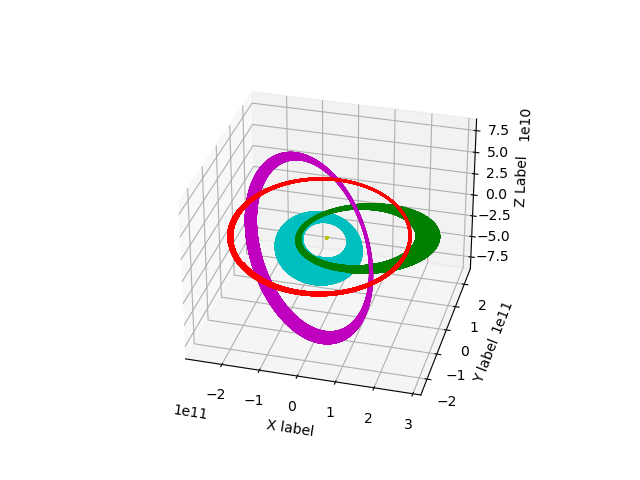
\includegraphics[width=0.4\columnwidth]{Euler Method/Euler Graph.png}}
        \subfloat[The Graph Produced using the Euler-Cromer Method]{
        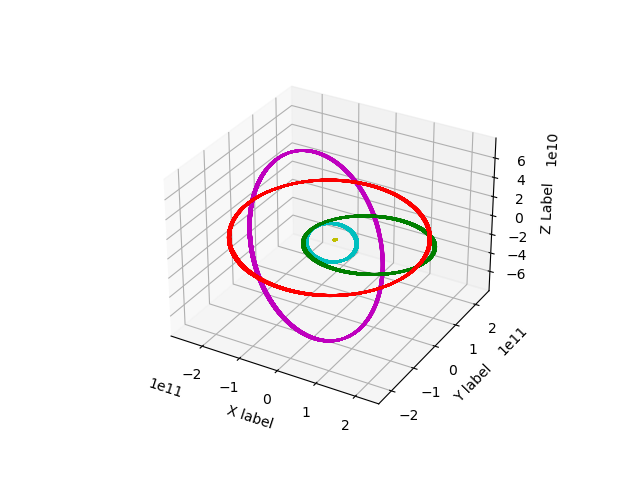
\includegraphics[width=0.4\columnwidth]{Euler-Cromer Method/Euler-Cromer Graph.png}}
        \caption{These plots were produced by the plotting function and are a 3 Dimension rendering of the movement of the bodies as taken in the 3,600-second time steps iterated 100,000 times. The Yellow Dot is a representation of the Sun, The Cyan Ellipse shows the orbit of Mercury, The magenta ellipse shows the orbit of Venus, The Green Ellipse shows the orbit of Earth and the Red ellipse shows the orbit of Mars}
        \label{plot:orbits}
     \end{figure}
 
 As Can be seen both the Euler and Euler-Cromer Methods got out the rough shape of the orbits of the different planets. This shows that although they could not predict perfectly the position of the planets when compared to the more precise and accurate model; that the simulation is still running an effective inner solar system and that both numerical methods have successfully produced the desired outcome of modelling the inner solar system's planetary bodies.



\newpage

\section{Conclusion}
\subsection{How the Model could have been improved}
This simulation could be improved via using a different numerical method. A Verlet algorithm or Runge-Kutta algorithm would have both have been more accurate than then the Euler and Euler-Cromer Methods used. Equally, if the intermediate Euler method had been used that would also have been more accurate than the Euler Method that was used by this simulation. These numerical approximations would have made the data more precise and would have led to the model being more able to predict its real world counterparts.

Equally, the Inclusion of the outer solar system is also something that could be improved upon. If the outer solar system's bodies had been included (which would have been possible as the Program works for an N bodied system), it would have meant that the simulation would be more precise as their gravitational pull affects the inner bodies and thus will cause errors that will make this simulation a lot less effective over longer periods of time

A further way this simulation could be improved is through the inclusion of some general relativity. If the simulation is to accurately predict the movement of the solar system the general relativity is needed to explain phenomena such as the Perihelion precession of Mercury's orbit. This may cause problems though as there would be a massive increase in the computational power and this may go out of the original parameters of the simulation

\subsection{Final Comments}
Overall the Model was successful in being able to reproduce the Order of magnitude of the Orbits as can be seen in Figures 2-4, although it was not able to accurately describe the exact position and velocity of the planets. Furthermore, the fact that the Change in Momentum and Energy in the system was so small it could be considered negligible shows that the system is also able to reproduce some universal conservations that weren't necessarily programmed in.The production of clear elliptical orbits mimicking those of actual planets also shows that the model has achieved some desired outcome.
\section{Bibliography}
\begin{thebibliography}{}
   
    \bibitem{Python} Rossum, Guido Van (20 January 2009). "The History of Python: A Brief Timeline of Python". The History of Python. Archived from the original on 5 June 2020. Retrieved 5 March 2021
   
    \bibitem{Euler} Bartuccelli, M., Deane, J., & Gentile, G. (2014). The high-order Euler method and the spin–orbit model. Celestial Mechanics and Dynamical Astronomy, 121(3), 233-260…
   
    \bibitem{Euler-Cromer} Chen, Z., & Gan, S. (2020). Convergence and stability of the backward Euler method for jump–diffusion SDEs with super-linearly growing diffusion and jump coefficients. Journal of Computational and Applied Mathematics, 363, 350-369.
       
    \bibitem{Universal Grav} DiLisi, G., & Morgan & Claypool Publishers, publisher. (2019). Classical mechanics. Volume 4, The universal law of gravitation (IOP (Series). Release 6). San Rafael [California] (40 Oak Drive, San Rafael, CA, 94903, USA): Morgan & ClaypoolDiLisi, G., & Morgan & Claypool Publishers, publisher. (2019). Classical mechanics. Volume 4, The universal law of gravitation (IOP (Series). Release 6). San Rafael [California] (40 Oak Drive, San Rafael, CA, 94903, USA): Morgan & Claypool
      
   \bibitem{university physics} Young H.D, Freedman R.A.University Physics with Modern Physics. Fifteenth Edition.A.L Ford, KZ Estrugo.Uni tied Kingdom:Pearson Education Limited,2020
   

    
    \bibitem{NumPy} Idris, I. (2012). NumPy cookbook. Birmingham, [Eng.]: Packt Publishing
    
    \bibitem{SLOM} An essay on Sir Isaac Newton's second law of motion. By the Reverend Mr. Ludlam. (1780). London.
    
    \bibitem {The earth moon system} M. Chapront-Touzé; J. Chapront (1983). "The lunar ephemeris ELP-2000". Astronomy & Astrophysics. 124: 54. Bibcode:1983A&A...124...50C
    
    \bibitem{taylor series} Dienes, P. (1957). The Taylor series; an introduction to the theory of functions of a complex variable. New York: Dover Publications.
    
    \bibitem{.npy}Idris, I. (2014). Python data analysis : Learn how to apply powerful data analysis techniques with popular open source Python modules (1st ed., Community experience distilled). Birmingham: Packt Publishing.
    
    \bibitem{QTIPlot}QtiPlot packages for Linux". pkgs.org. Retrieved 26 April 2015.
\end{thebibliography}

\end{document}